\let\negmedspace\undefined
\let\negthickspace\undefined
\documentclass[journal]{IEEEtran}
\usepackage[a5paper, margin=10mm, onecolumn]{geometry}
%\usepackage{lmodern} % Ensure lmodern is loaded for pdflatex
\usepackage{tfrupee} % Include tfrupee package

\setlength{\headheight}{1cm} % Set the height of the header box
\setlength{\headsep}{0mm}     % Set the distance between the header box and the top of the text

\usepackage{gvv-book}
\usepackage{gvv}
\usepackage{cite}
\usepackage{amsmath,amssymb,amsfonts,amsthm}
\usepackage{algorithmic}
\usepackage{graphicx}
\usepackage{textcomp}
\usepackage{xcolor}
\usepackage{txfonts}
\usepackage{listings}
\usepackage{enumitem}
\usepackage{mathtools}
\usepackage{gensymb}
\usepackage{comment}
\usepackage[breaklinks=true]{hyperref}
\usepackage{tkz-euclide} 
\usepackage{listings}
% \usepackage{gvv}                                        
\def\inputGnumericTable{}                                 
\usepackage[latin1]{inputenc}                                
\usepackage{color}                                            
\usepackage{array}                                            
\usepackage{longtable}                                       
\usepackage{calc}                                             
\usepackage{multirow}                                         
\usepackage{hhline}                                           
\usepackage{ifthen}                                           
\usepackage{lscape}
\usepackage{circuitikz}
\tikzstyle{block} = [rectangle, draw, fill=blue!20, 
    text width=4em, text centered, rounded corners, minimum height=3em]
\tikzstyle{sum} = [draw, fill=blue!10, circle, minimum size=1cm, node distance=1.5cm]
\tikzstyle{input} = [coordinate]
\tikzstyle{output} = [coordinate]


\begin{document}

\bibliographystyle{IEEEtran}
\vspace{3cm}

\title{2.2.30}
\author{AI25BTECH11037-stalin}
 \maketitle
% \newpage
% \bigskip
{\let\newpage\relax\maketitle}
\renewcommand{\thefigure}{\theenumi}
\renewcommand{\thetable}{\theenumi}
\setlength{\intextsep}{10pt} % Space between text and floats
\numberwithin{equation}{enumi}
\numberwithin{figure}{enumi}
\renewcommand{\thetable}{\theenumi}
\textbf{Question}:\\
 Find the angle between the line 
\begin{align}
\frac{x+1}{2} = \frac{y}{3} = \frac{z-3}{6}
\end{align}
and the plane 
\begin{align}
10x + 2y - 11z = 3.
\end{align}

.\\
\solution \\
Let us solve the given equation theoretically and then verify the solution computationally \\
According to the question, \\
Given a plane and line\\
Let $\theta$ be angle between plane and line\\
Then $90^\circ-\theta$ is angle between normal vector of plane and line\\
Let $\vec{D}$ be dirction vector of line and $\vec{n}$ be normal of plane\\
\begin{align}
\vec{D}=\begin{myvec}{2\\3\\6}\end{myvec}\
\vec{n}=\begin{myvec}{10\\2\\-11}\end{myvec}\
\end{align}
\begin{align}
   \cos(90^\circ-\theta)=\frac{\vec{D}^T\vec{n}}{\|\vec{n}\|\|\vec{D}\|}=\frac{-8}{21}
\end{align}
\begin{align}
    \theta=90^\circ-\cos^{-1} (\frac{-8}{21})=-22.39^\circ
\end{align}
angle is $22.39^\circ$
\begin{figure}[h!]
    \centering
    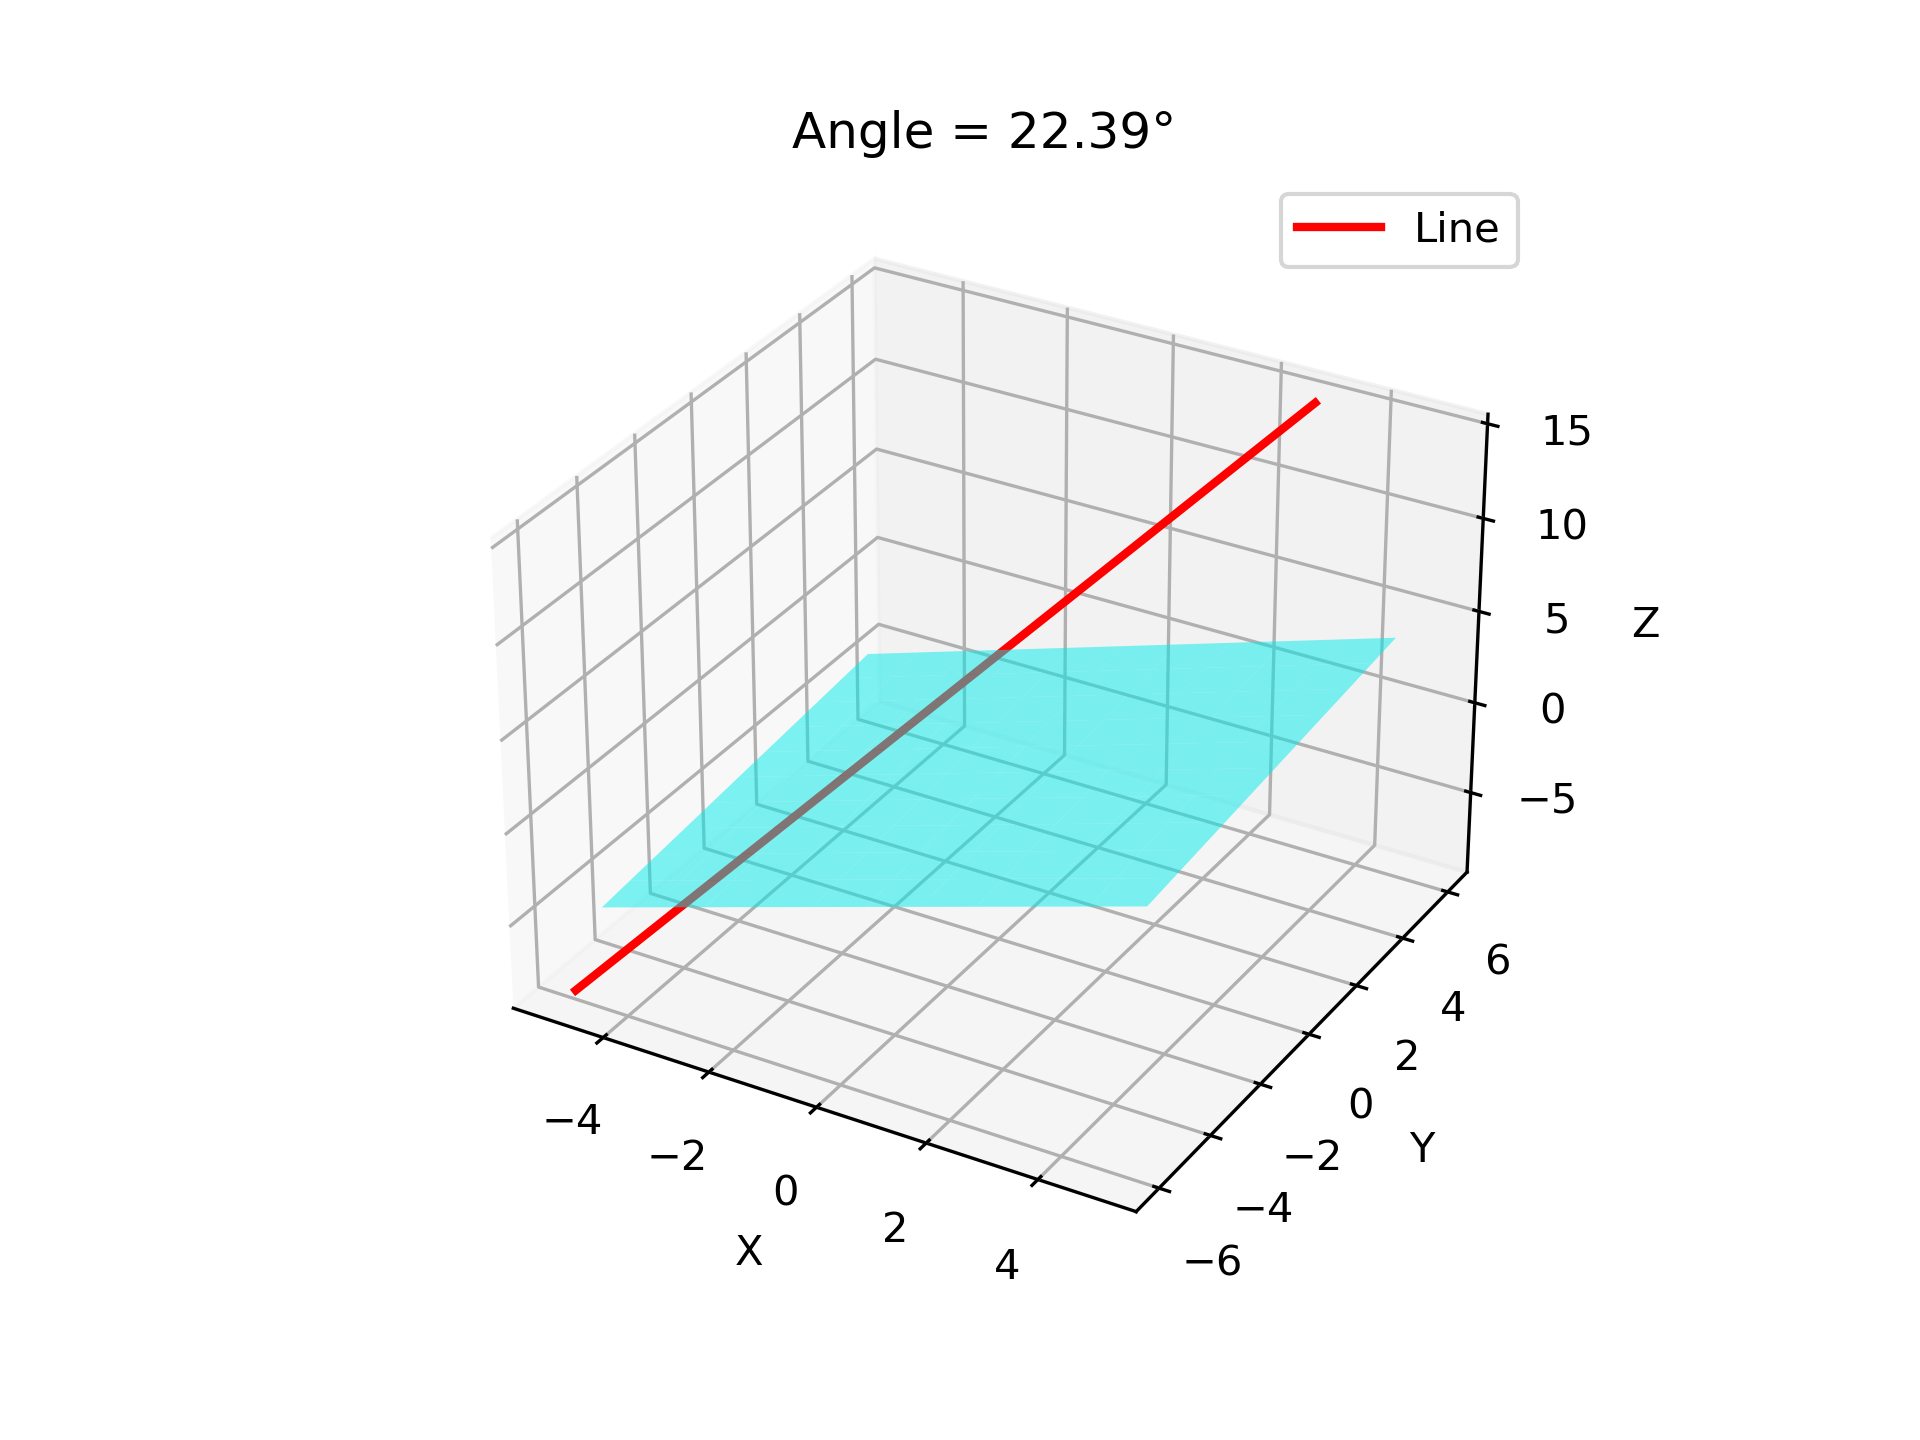
\includegraphics[width=0.8\columnwidth]{figs/line_plane_angle.png}
    \caption{}
    \label{fig:placeholder}
\end{figure}
\end{document}